\documentclass[dvipdfmx,11pt]{beamer}

\usepackage[deluxe]{otf} 
\usepackage{txfonts}
\renewcommand{\kanjifamilydefault}{\gtdefault}
\usepackage{amssymb,amsmath}
\usepackage{hyperref}
\usepackage[absolute,overlay]{textpos}
\usepackage{comment}
\usepackage{colortbl}
\usepackage{graphicx}
\usepackage{tikz}
\usetikzlibrary{positioning}
\usetikzlibrary{shadows}
\usetikzlibrary{calc}
\usepackage{listings}
\usepackage{plistings}
\usepackage{multicol}
\usepackage{multirow}
\usepackage{caption}
\def\lstlistingname{コード}
\lstset{escapeinside=||}
\newcommand{\code}[1]{\lstinline[basicstyle=\ttfamily]{#1}}
\newcommand{\lw}[1]{\smash{\lower-5.ex\hbox{#1}}}
\newcommand{\redunderline}[1]{\textcolor{red}{\underline{\textcolor{black}{#1}}}}
%%\usetheme{Frankfurt}
\usetheme{Warsaw}
\setbeamertemplate{navigation symbols}{} %スライドのボタン?(右下のやつ)を消す
\setbeamersize{text margin left=1.5em,text margin right=1.5em} % 余白なくすやつ

% footer setting %
\makeatother
\setbeamertemplate{footline}
{
  \leavevmode%
  \hbox{%
  \begin{beamercolorbox}[wd=.4\paperwidth,ht=2.25ex,dp=1ex,center]{author in head/foot}%
    \usebeamerfont{author in head/foot}\insertshortauthor
  \end{beamercolorbox}%
  \begin{beamercolorbox}[wd=.6\paperwidth,ht=2.25ex,dp=1ex,center]{title in head/foot}%
    \usebeamerfont{title in head/foot}\hspace*{1ex} \insertshorttitle\hspace*{3em}
    \textbf{ \insertframenumber{} / \inserttotalframenumber } \hspace*{1ex}
  \end{beamercolorbox}}%
  \vskip0pt%
}
\makeatletter

% exclude apprendix slides from framenumber %
\newcommand{\backupbegin}{
   \newcounter{framenumberappendix}
   \setcounter{framenumberappendix}{\value{framenumber}}
}
\newcommand{\backupend}{
   \addtocounter{framenumberappendix}{-\value{framenumber}}
   \addtocounter{framenumber}{\value{framenumberappendix}} 
}

\lstset{
 basicstyle=\ttfamily\color{black},
 keepspaces=true,
 escapechar=|,
 columns=[l]{fullflexible},
 commentstyle={\color{red}},
 stringstyle={\color{blue}}}

\title{解集合プログラミングを用いた\\配電網問題の解法}
\author[山田 健太郎,湊 真一,田村 直之,番原 睦則]
{山田 健太郎$^1$,湊 真一$^2$,田村 直之$^3$,番原 睦則$^1$}
\date{第24回プログラミングおよびプログラミング言語ワークショップ}
\institute{1.名古屋大学 大学院情報学研究科\\
2.京都大学 大学院情報学研究科\\
3.神戸大学 情報基盤センター
}

%#################################################
%# 本文 ##########################################
%#################################################
\begin{document}

%%%%%%%%%%%%%%%%%%%%%%%%%%%%%%%%%%%%%%%%%%%%%%%%%%
%% タイトル 
%%%%%%%%%%%%%%%%%%%%%%%%%%%%%%%%%%%%%%%%%%%%%%%%%%
\begin{frame}{}
  \titlepage
\end{frame}

%%%%%%%%%%%%%%%%%%%%%%%%%%%%%%%%%%%%%%%%%%%%%%%%%%
% 配電網
%%%%%%%%%%%%%%%%%%%%%%%%%%%%%%%%%%%%%%%%%%%%%%%%%%
\begin{frame}{配電網問題}
  \begin{alertblock}{}\centering
    求解困難な組合せ最適化問題の一種
  \end{alertblock}
  \vfill
  \begin{itemize}
  \item \alert{\bf 配電網}とは,変電所と,一般家庭や工場を繋ぐ電力供給
    経路のネットワークである.
  \item  配電網の構成技術はスマートグリッドや,災害時の停電復旧
         などを支える重要な基盤技術として期待されている.
  \item \alert{\bf 配電網問題}とは,
    \begin{itemize}
    \item \structure{\bf トポロジ制約}と\structure{\bf 電気制約}を満たしつつ,
    \item 損失電力を最小にするスイッチの開閉状態を求めることが目的.
    \end{itemize}
  \item これまで,メタヒューリスティクス等の解法が提案されている.
  \item 厳密解法として,フロンティア法を用いた解法が提案されている.
    \begin{itemize}
    \item 実用規模の配電網問題(\structure{\textsf{\bf fukui-tepco},\textbf{スイッチ数468個}})の
      最適解を求めることに成功~[井上ほか '12].
    \end{itemize}
  \end{itemize}
\end{frame}
%%%%%%%%%%%%%%%%%%%%%%%%%%%%%%%%%%%%%%%%%%%%%%%%%%
%% 解の遷移問題
%%%%%%%%%%%%%%%%%%%%%%%%%%%%%%%%%%%%%%%%%%%%%%%%%%
\begin{frame}{配電網遷移問題}
 \begin{alertblock}{配電網遷移問題}
  配電網問題とその2つの実行可能解が与えられたとき,
  一方の解から他方の解へ,\alert{\bf 遷移制約}を満たしつつ,
  実行可能解のみを経由して到達できるかどうかを判定する問題.
  \begin{itemize}
  \item 各ステップ$t$で変更可能なスイッチを$d$個に制限.(\textbf{遷移制約})
  \item 本研究では,到達可能であればその最短経路を求めることが目的.
  %\item 最短ステップ長での辺の変更手順を求めることが目的となる.
  \end{itemize}
 \end{alertblock}
 \begin{itemize}
  \item 配電網の構成制御における災害時の停電復旧などへの応用が狙い.
  \item 近年,理論計算機科学の分野を中心に急速に発展している
        \structure{\bf 組合せ遷移問題}の一種.
 \end{itemize}
 \begin{alertblock}{}\centering
  しかし現状では,配電網遷移問題を効率的に解くソルバーの \\
  \alert{\bf 実装技術は確立されていない}.
 \end{alertblock}
\end{frame}
%%%%%%%%%%%%%%%%%%%%%%%%%%%%%%%%%%%%%%%%%%%%%%%%%%
%% 遷移問題の例
%%%%%%%%%%%%%%%%%%%%%%%%%%%%%%%%%%%%%%%%%%%%%%%%%%
\begin{frame}{配電網遷移問題の例}
  \renewcommand{\thefootnote}{\fnsymbol{footnote}}
  \setcounter{footnote}{1}
  \begin{columns}
    \begin{column}{0.45\textwidth}\centering
      \begin{exampleblock}{スタート状態}
    \centering
    \scalebox{0.35}{\begin{tikzpicture}

 % setting
 \tikzset{customer/.style={rectangle,thick,draw=black,minimum size=0.5cm}}
 \tikzset{on_switch/.style={rectangle,fill=black}}
 \tikzset{off_switch/.style={rectangle,draw=black,fill=white}}
 
 \tikzset{node distance =1cm};

 % substation (x, y, label)
 \newcommand{\substation}[3]{
 \draw [very thick] (#1,#2) circle [radius=0.225cm] node[draw=none,minimum size=1cm](#3){};
 \draw [very thick] (#1+0.225,#2)--(#1+0.35,#2)--(#1+0.35,#2+0.3);
 \draw [very thick] (#1-0.225,#2)--(#1-0.35,#2)--(#1-0.35,#2-0.3);
 \draw [very thick] (#1,#2+0.225)--(#1,#2+0.35);
 \draw [very thick] (#1,#2-0.225)--(#1,#2-0.35);
 \draw [very thick] [domain=-0.284:-0.159] plot(\x+#1,\x+#2);
 \draw [very thick] [domain=0.159:0.284] plot(\x+#1,\x+#2);
 \draw [very thick] [domain=-0.284:-0.159] plot(\x+#1,-\x+#2);
 \draw [very thick] [domain=0.159:0.284] plot(\x+#1,-\x+#2);
 }

 %switch node (position, label, cap)
 %% right switch
 \newcommand{\swnodeR}[4]{
 \coordinate[#1] (#2);
 \node[#1,customer] (#2){#4};
 \node[circle, draw=black, text width=0.2cm, 
 right=0cm of #2, scale=0.3, thick] {};
 \node[right=0cm of #2,scale=0.3, minimum size=0.8cm] (#3){};
 }
 %% left switch
 \newcommand{\swnodeL}[4]{
 %\coordinate[#1] (#2);
 \node[#1,customer] (#2){#4};
 \node[circle, draw=black, fill=white, text width=0.2cm, 
 left=0cm of #2, scale=0.3, thick] (#3){};
 }
 % above switch
 \newcommand{\swnodeA}[4]{
 \coordinate[#1] (#2);
 \node[#1,customer] (#2){#4};
 \node[circle, draw=black, text width=0.2cm, 
 above=0cm of #2, scale=0.3, thick] (#3){};
 }
 % below switch
 \newcommand{\swnodeB}[4]{
 \coordinate[#1] (#2);
 \node[#1,customer] (#2){#4};
 \node[circle, draw=black, text width=0.2cm, 
 below=0cm of #2, scale=0.3, thick] {};
 \node[below=0cm of #2,scale=0.3,minimum size=0.8cm] (#3){};
 }
 
 \substation{0}{0}{sub};
 
 % root1
 \node[customer,fill=purple!60,below =4.5cm of sub] (root1) { };
 \swnodeL{left =of root1,fill=purple!60}{node1}{sw1}{ };
 
 \swnodeR{left=of node1,fill=purple!60}{node2}{sw2}{ };
 \node[customer,left=of node2,fill=purple!60] (junc1){ };
 \swnodeL{left =of junc1,fill=purple!60}{node3}{sw3}{ };
 \swnodeA{above= of junc1,fill=purple!60}{node4}{sw4}{ }

 \swnodeR{left=of node3,fill=purple!60}{node5}{sw5}{ };
 \swnodeA{above =of node5,fill=purple!60}{node6}{sw6}{ };

 \swnodeB{above =of node6,fill=cyan!80}{node7}{sw7}{ };
 \swnodeA{above =of node7,fill=cyan!80}{node29}{sw29}{ };

 \swnodeB{above =of node29,fill=cyan!80}{node30}{sw30}{ };
 
 \swnodeB{above =of node4,fill=purple!60}{node8}{sw8}{ };
 \swnodeA{above =of node8,fill=purple!60}{node31}{sw31}{ };
 
 \swnodeB{above =of node31,fill=cyan!80}{node32}{sw32}{ };

 \swnodeR{right =of root1,fill=purple!60}{node17}{sw17}{ };

 \swnodeL{right =of node17,fill=purple!60}{node18}{sw18}{ };

 % root2
 \node[customer,fill=black!20,above=4.5cm of sub, fill=cyan!80] (root2) { };
 \swnodeL{left =of root2,fill=cyan!80}{node9}{sw9}{ };

 \swnodeR{left=of node9,fill=cyan!80}{node10}{sw10}{ };
 \node[customer,left=of node10,fill=cyan!80] (junc2){ };
 \swnodeL{left =of junc2,fill=cyan!80}{node11}{sw11}{ };
 \swnodeB{below =of junc2,fill=cyan!80}{node12}{sw12}{ };
 
 \swnodeR{left =of node11,fill=cyan!80}{node13}{sw13}{ };
 \swnodeB{below =of node13,fill=cyan!80}{node14}{sw14}{ };
 
 \swnodeA{below =of node14,fill=cyan!80}{node15}{sw15}{ };

 \swnodeA{below =of node12,fill=cyan!80}{node16}{sw16}{ };

 \swnodeR{right =of root2,fill=cyan!80}{node22}{sw22}{ };

 \swnodeL{right =of node22,fill=cyan!80}{node23}{sw23}{ };
 
 % root3
 \node[customer,fill=black!20,right=5.2cm of sub,fill=yellow!80] (root3) { };
 \swnodeB{below =1.4of root3,fill=yellow!80}{node24}{sw24}{ };
 \swnodeA{above =1.4of root3,fill=yellow!80}{node25}{sw25}{ };

 \swnodeA{below =of node24,fill=yellow!80}{node19}{sw19}{ };
 \swnodeL{below =1.3of node19,fill=yellow!80}{node20}{sw20}{ };
 
 \swnodeR{left =of node20,fill=purple!60}{node21}{sw21}{ };

 \swnodeB{above =of node25,fill=yellow!80}{node26}{sw26}{ };
 \swnodeL{above =1.3of node26,fill=yellow!80}{node27}{sw27}{ };

 \swnodeR{left =of node27,fill=cyan!80}{node28}{sw28}{ };
 
 % sections
 \foreach \v / \u / \t in {root1/sub/$s_a$,root1/node1/$s_1$,node2/junc1/$s_2$, %
 junc1/node3/$s_3$,junc1/node4/$s_4$,node5/node6/$s_5$,node7/node29/$s_6$,node30/node15/$s_7$, %
 sub/root2/$s_b$,root2/node9/$s_8$,node10/junc2/$s_9$,junc2/node11/$s_{10}$,node12/junc2/$s_{11}$, %
 node14/node13/$s_{12}$,node8/node31/$s_{13}$,node32/node16/$s_{14}$,node17/root1/$s_{15}$, %
 node22/root2/$s_{16}$,root3/sub/$s_c$,node24/root3/$s_{17}$,root3/node25/$s_{18}$, %
 node20/node19/$s_{19}$,node26/node27/$s_{20}$,node21/node18/$s_{21}$,node28/node23/$s_{22}$} %
 \draw[thick] (\v) --  node[auto=right]{\t} (\u);

 % switches
 %% horizontal
 \foreach \v / \u / \t in {sw1/sw2/$sw_{1}$,sw3/sw5/$sw_{2}$,sw9/sw10/$sw_{11}$,
 sw11/sw13/$sw_{12}$,sw18/sw17/$sw_{13}$,sw23/sw22/$sw_{15}$}
 \draw[very thick] (\v) -- node[below=0.2of \v]{\t} (\u.center);
 
 \foreach \v / \u in {sw20/sw21,sw27/sw28}
 \draw[very thick] (\v) -- (\u.45);
 %% vertical
 \foreach \v / \u / \t in {sw4/sw8/$sw_{4}$,sw29/sw30/$sw_{5}$,sw15/sw14/$sw_{7}$,%
 sw16/sw12/$sw_{8}$,sw19/sw24/$sw_{9}$,sw25/sw26/$sw_{10}$}
 \draw[very thick] (\v) -- node[auto=below]{\t~~~~~~~~~~} (\u.center);

 \foreach \v / \u in {sw6/sw7,sw31/sw32}
 \draw[very thick] (\v) -- (\u.-30);

 \coordinate[above=0.5of node7](A);
 \coordinate[above=0.3of node26](B);
 \coordinate[above=0.8of node20](C);
 \draw[ultra thick, draw=blue, densely dotted] (A) circle[x radius=0.8,y radius=2.2];
 \draw[ultra thick, draw=red, densely dotted] (B) circle[x radius=0.8,y radius=1.8];
 \draw[ultra thick, draw=teal, densely dotted] (C) circle[x radius=0.8,y radius=1.8];

\end{tikzpicture}

%%%%%%%%%%%%%%%%%%%%%%%%%%%%%%%%%%%%%%%%%%%%%%%%%%%%%%%%%%
%%% Local Variables:
%%% mode: japanese-latex
%%% TeX-master: paper.tex
%%% End:
}
      \end{exampleblock}
    \end{column}
    \begin{column}{0.05\textwidth}\centering
      $\Rightarrow$
    \end{column}
    \begin{column}{0.45\textwidth}\centering
      \begin{exampleblock}{ゴール状態}
        \centering
        \scalebox{0.35}{\begin{tikzpicture}

 % setting
 \tikzset{customer/.style={rectangle,thick,draw=black,minimum size=0.5cm}}
 \tikzset{on_switch/.style={rectangle,fill=black}}
 \tikzset{off_switch/.style={rectangle,draw=black,fill=white}}
 
 \tikzset{node distance =1cm};

 % substation (x, y, label)
 \newcommand{\substation}[3]{
 \draw [very thick] (#1,#2) circle [radius=0.225cm] node[draw=none,minimum size=1cm](#3){};
 \draw [very thick] (#1+0.225,#2)--(#1+0.35,#2)--(#1+0.35,#2+0.3);
 \draw [very thick] (#1-0.225,#2)--(#1-0.35,#2)--(#1-0.35,#2-0.3);
 \draw [very thick] (#1,#2+0.225)--(#1,#2+0.35);
 \draw [very thick] (#1,#2-0.225)--(#1,#2-0.35);
 \draw [very thick] [domain=-0.284:-0.159] plot(\x+#1,\x+#2);
 \draw [very thick] [domain=0.159:0.284] plot(\x+#1,\x+#2);
 \draw [very thick] [domain=-0.284:-0.159] plot(\x+#1,-\x+#2);
 \draw [very thick] [domain=0.159:0.284] plot(\x+#1,-\x+#2);
 }

 %switch node (position, label, cap)
 %% right switch
 \newcommand{\swnodeR}[4]{
 \coordinate[#1] (#2);
 \node[#1,customer] (#2){#4};
 \node[circle, draw=black, text width=0.2cm, 
 right=0cm of #2, scale=0.3, thick] {};
 \node[right=0cm of #2,scale=0.3, minimum size=0.8cm] (#3){};
 }
 %% left switch
 \newcommand{\swnodeL}[4]{
 %\coordinate[#1] (#2);
 \node[#1,customer] (#2){#4};
 \node[circle, draw=black, fill=white, text width=0.2cm, 
 left=0cm of #2, scale=0.3, thick] (#3){};
 }
 % above switch
 \newcommand{\swnodeA}[4]{
 \coordinate[#1] (#2);
 \node[#1,customer] (#2){#4};
 \node[circle, draw=black, text width=0.2cm, 
 above=0cm of #2, scale=0.3, thick] (#3){};
 }
 % below switch
 \newcommand{\swnodeB}[4]{
 \coordinate[#1] (#2);
 \node[#1,customer] (#2){#4};
 \node[circle, draw=black, text width=0.2cm, 
 below=0cm of #2, scale=0.3, thick] {};
 \node[below=0cm of #2,scale=0.3,minimum size=0.8cm] (#3){};
 }
 
 \substation{0}{0}{sub};
 
 % root1
 \node[customer,fill=purple!60,below =4.5cm of sub] (root1) { };
 \swnodeL{left =of root1,fill=purple!60}{node1}{sw1}{ };
 
 \swnodeR{left=of node1,fill=purple!60}{node2}{sw2}{ };
 \node[customer,left=of node2,fill=purple!60] (junc1){ };
 \swnodeL{left =of junc1,fill=purple!60}{node3}{sw3}{ };
 \swnodeA{above= of junc1,fill=purple!60}{node4}{sw4}{ }

 \swnodeR{left=of node3,fill=purple!60}{node5}{sw5}{ };
 \swnodeA{above =of node5,fill=purple!60}{node6}{sw6}{ };

 \swnodeB{above =of node6,fill=purple!60}{node7}{sw7}{ };
 \swnodeA{above =of node7,fill=purple!60}{node29}{sw29}{ };

 \swnodeB{above =of node29,fill=cyan!80}{node30}{sw30}{ };
 
 \swnodeB{above =of node4,fill=purple!60}{node8}{sw8}{ };
 \swnodeA{above =of node8,fill=purple!60}{node31}{sw31}{ };
 
 \swnodeB{above =of node31,fill=cyan!80}{node32}{sw32}{ };

 \swnodeR{right =of root1,fill=purple!60}{node17}{sw17}{ };

 \swnodeL{right =of node17,fill=purple!60}{node18}{sw18}{ };

 % root2
 \node[customer,fill=cyan!80,above=4.5cm of sub, fill=cyan!80] (root2) { };
 \swnodeL{left =of root2,fill=cyan!80}{node9}{sw9}{ };

 \swnodeR{left=of node9,fill=cyan!80}{node10}{sw10}{ };
 \node[customer,left=of node10,fill=cyan!80] (junc2){ };
 \swnodeL{left =of junc2,fill=cyan!80}{node11}{sw11}{ };
 \swnodeB{below =of junc2,fill=cyan!80}{node12}{sw12}{ };
 
 \swnodeR{left =of node11,fill=cyan!80}{node13}{sw13}{ };
 \swnodeB{below =of node13,fill=cyan!80}{node14}{sw14}{ };
 
 \swnodeA{below =of node14,fill=cyan!80}{node15}{sw15}{ };

 \swnodeA{below =of node12,fill=cyan!80}{node16}{sw16}{ };

 \swnodeR{right =of root2,fill=cyan!80}{node22}{sw22}{ };

 \swnodeL{right =of node22,fill=cyan!80}{node23}{sw23}{ };
 
 % root3
 \node[customer,fill=cyan!80,right=5.2cm of sub,fill=yellow!80] (root3) { };
 \swnodeB{below =1.4of root3,fill=yellow!80}{node24}{sw24}{ };
 \swnodeA{above =1.4of root3,fill=yellow!80}{node25}{sw25}{ };

 \swnodeA{below =of node24,fill=purple!60}{node19}{sw19}{ };
 \swnodeL{below =1.3of node19,fill=purple!60}{node20}{sw20}{ };
 
 \swnodeR{left =of node20,fill=purple!60}{node21}{sw21}{ };

 \swnodeB{above =of node25,fill=cyan!80}{node26}{sw26}{ };
 \swnodeL{above =1.3of node26,fill=cyan!80}{node27}{sw27}{ };

 \swnodeR{left =of node27,fill=cyan!80}{node28}{sw28}{ };
 
 % sections
 \foreach \v / \u / \t in {root1/sub/$s_a$,root1/node1/$s_1$,node2/junc1/$s_2$, %
 junc1/node3/$s_3$,junc1/node4/$s_4$,node5/node6/$s_5$,node7/node29/$s_6$,node30/node15/$s_7$, %
 sub/root2/$s_b$,root2/node9/$s_8$,node10/junc2/$s_9$,junc2/node11/$s_{10}$,node12/junc2/$s_{11}$, %
 node14/node13/$s_{12}$,node8/node31/$s_{13}$,node32/node16/$s_{14}$,node17/root1/$s_{15}$, %
 node22/root2/$s_{16}$,root3/sub/$s_c$,node24/root3/$s_{17}$,root3/node25/$s_{18}$, %
 node20/node19/$s_{19}$,node26/node27/$s_{20}$,node21/node18/$s_{21}$,node28/node23/$s_{22}$} %
 \draw[thick] (\v) --  node[auto=right]{\t} (\u);

 % switches
 %% horizontal
 \foreach \v / \u / \t in {sw1/sw2/$sw_{1}$,sw3/sw5/$sw_{2}$,sw9/sw10/$sw_{11}$,
 sw11/sw13/$sw_{12}$,sw18/sw17/$sw_{13}$,sw20/sw21/$sw_{14}$,sw23/sw22/$sw_{15}$,
 sw27/sw28/$sw_{16}$}
 \draw[very thick] (\v) -- node[below=0.2of \v]{\t} (\u.center);
 
 % \foreach \v / \u in {}
 % \draw[very thick] (\v) -- (\u.45);
 %% vertical
 \foreach \v / \u / \t in {sw4/sw8/$sw_{4}$,sw6/sw7/$sw_{3}$,sw15/sw14/$sw_{7}$,%
 sw16/sw12/$sw_{8}$}
 \draw[very thick] (\v) -- node[auto=below]{\t~~~~~~~~~~} (\u.center);

 \foreach \v / \u in {sw29/sw30,sw31/sw32,sw25/sw26,sw19/sw24}
 \draw[very thick] (\v) -- (\u.-30);

 \coordinate[above=0.5of node7](A);
 \coordinate[above=0.3of node26](B);
 \coordinate[above=0.8of node20](C);
 \draw[ultra thick, draw=blue, densely dotted] (A) circle[x radius=0.8,y radius=2.2];
 \draw[ultra thick, draw=red, densely dotted] (B) circle[x radius=0.8,y radius=1.8];
 \draw[ultra thick, draw=teal, densely dotted] (C) circle[x radius=0.8,y radius=1.8];

\end{tikzpicture}

%%%%%%%%%%%%%%%%%%%%%%%%%%%%%%%%%%%%%%%%%%%%%%%%%%%%%%%%%%
%%% Local Variables:
%%% mode: japanese-latex
%%% TeX-master: paper.tex
%%% End:
}
      \end{exampleblock}
    \end{column}
  \end{columns}
 \vfill
 \begin{itemize}
  \item セクション数:25個,スイッチ数:16個,変電所数:3個\footnote{%
        変電所に直接つながるセクションの数}%
  \item 各ステップで変更可能なスイッチを2個に制限.(\textbf{遷移制約})
  \item スタート状態からゴール状態へ\structure{\bf 3ステップで到達可能}.
 \end{itemize}
\end{frame}
%%%%%%%%%%%%%%%%%%%%%%%%%%%%%%%%%%%%%%%%%%%%%%%%%%
%% ASP
%%%%%%%%%%%%%%%%%%%%%%%%%%%%%%%%%%%%%%%%%%%%%%%%%%
\begin{frame}{解集合プログラミング(Answer Set Programming; ASP)}
\vfill
 \begin{itemize}
  \item \structure{\bf ASPの言語}は一階論理に基づく知識表現言語の一種である.
  \item \structure{\bf ASPシステム}は論理プログラムから安定モデル意味
        論~[Gelfond and Lifschitz '88]に基づく解集合を計算するシステムである.
  \item 近年,SATソルバーの実装技術を応用した高速ASPシステムが実現され,
        システム検証,プランニング,システム生物学など様々な分野への応用が
        拡大している.
 \end{itemize}
 \vfill
 \begin{alertblock}{配電網遷移問題に対してASP技術を用いる利点}
  \begin{itemize}
   \item ASP言語の高い表現力を活かし,組合せ問題を\textbf{簡潔に記述可能}
         \begin{itemize}
          \item \alert{\bf 組合せ遷移問題への拡張も容易}
         \end{itemize}
   \item マルチショットASP解法により,ステップ長を増やしながら,組合せ遷移問題の
         \alert{\bf 到達可能性を効率的に検査可能}
         \begin{itemize}
          \item ASPシステムを複数回起動するオーバヘッドを回避可能
          \item 同様の探索失敗を避けるために獲得した学習節を再利用可能
         \end{itemize}
  \end{itemize}
 \end{alertblock} \vfill
\end{frame}
%%%%%%%%%%%%%%%%%%%%%%%%%%%%%%%%%%%%%%%%%%%%%%%%%%
%% 研究目的
%%%%%%%%%%%%%%%%%%%%%%%%%%%%%%%%%%%%%%%%%%%%%%%%%%
\begin{frame}{研究目的}
  \begin{alertblock}{目的}
   ASP技術を活用した大規模な配電網遷移問題を効率良く解くシステムを構築
   する.
  \end{alertblock}
  \vfill
 \begin{block}{研究内容}
  \begin{enumerate}
   \item \structure{\bf 配電網問題のASP符号化の考案}
         \begin{itemize}
          \item トポロジ制約のASP符号化として,\textbf{基本符号化},\textbf{改良符号化},
                \\ \alert{\bf 有向符号化} の3種類を考案.
          \item 電気制約として,電流制約のASP符号化を考案.
         \end{itemize}
   \item \structure{\bf 配電網遷移問題のASP符号化の考案}
         \begin{itemize}
          \item \textbf{シングルショット符号化}と\alert{\bf マルチショット符号化}の2種類を考案.
          \item 配電網問題のASP符号化の自然な拡張である.
         \end{itemize}
   \item \structure{\bf 実用規模の問題を含むベンチマークによる評価実験}
         \begin{itemize}
          \item 実用規模の問題である\textsf{fukui-tepco}をもとに,
                配電網遷移問題ベンチマークを1000問作成.
          \item \textbf{マルチショット符号化}は,
                \alert{\bf 約3.8倍の高速化}を実現.
         \end{itemize}
  \end{enumerate}
 \end{block}
\end{frame}
%%%%%%%%%%%%%%%%%%%%%%%%%%%%%%%%%%%%%%%%%%%%%%%%%%
%% トポロジ制約
%%%%%%%%%%%%%%%%%%%%%%%%%%%%%%%%%%%%%%%%%%%%%%%%%%
\begin{frame}{~}
 \LARGE \centering
 \structure{\bf 配電網問題}
\end{frame}
%
\begin{frame}[noframenumbering]{配電網問題のトポロジ制約}
 \begin{alertblock}{}
  トポロジ制約を満たす配電網構成は,グラフと根と呼ばれる特別なノードから,
  \alert{\bf 根付き全域森}を求める部分グラフ探索問題に帰着できる.
 \end{alertblock}
 \vfill
 \begin{block}{根付き全域森 (Spanning Rooted Forest) [川原・湊 '12]}
  グラフ$G=(V,E)$と,
  \textbf{根}と呼ばれる$V$上のノードが与えられたとき,
  $G$上の根付き全域森とは,以下の条件を満たす$G$の部分グラフ$G'=(V,E'),\ E' \subseteq E$である.
  \begin{enumerate}
   \item $G'$はサイクルを持たない. (\alert{\bf 非閉路制約})
   \item $G'$の各連結成分は,ちょうど1つの根を含む. (\alert{\bf 根付き連結制約})
  \end{enumerate}
 \end{block}
\end{frame}
%%%%%%%%%%%%%%%%%%%%%%%%%%%%%%%%%%%%%%%%%%%%%%%%%%
%% トポロジ制約の例
%%%%%%%%%%%%%%%%%%%%%%%%%%%%%%%%%%%%%%%%%%%%%%%%%%
\begin{frame}{配電網問題のトポロジ制約}
  \renewcommand{\thefootnote}{\fnsymbol{footnote}}
  \setcounter{footnote}{1}
  \begin{columns}
    \begin{column}{0.45\textwidth}\centering
      \begin{exampleblock}{配電網問題の解}
    \centering
    \scalebox{0.3}{%%%%%%%%%%%%%%%%%%%%%%%%%%%%%%%%%%%%%%%%%%%%%%%%%%
% 配電網 例 (第1章で使う)
%%%%%%%%%%%%%%%%%%%%%%%%%%%%%%%%%%%%%%%%%%%%%%%%%%

\begin{tikzpicture}

 % setting
 \tikzset{customer/.style={rectangle,thick,draw=black,minimum size=0.5cm}}
 \tikzset{on_switch/.style={rectangle,fill=black}}
 \tikzset{off_switch/.style={rectangle,draw=black,fill=white}}
 
 \tikzset{node distance =1cm};

 % substation (x, y, label)
 \newcommand{\substation}[3]{
 \draw [very thick] (#1,#2) circle [radius=0.225cm] node[draw=none,minimum size=1cm](#3){};
 \draw [very thick] (#1+0.225,#2)--(#1+0.35,#2)--(#1+0.35,#2+0.3);
 \draw [very thick] (#1-0.225,#2)--(#1-0.35,#2)--(#1-0.35,#2-0.3);
 \draw [very thick] (#1,#2+0.225)--(#1,#2+0.35);
 \draw [very thick] (#1,#2-0.225)--(#1,#2-0.35);
 \draw [very thick] [domain=-0.284:-0.159] plot(\x+#1,\x+#2);
 \draw [very thick] [domain=0.159:0.284] plot(\x+#1,\x+#2);
 \draw [very thick] [domain=-0.284:-0.159] plot(\x+#1,-\x+#2);
 \draw [very thick] [domain=0.159:0.284] plot(\x+#1,-\x+#2);
 }

 %switch node (position, label, cap)
 %% right switch
 \newcommand{\swnodeR}[4]{
 \coordinate[#1] (#2);
 \node[#1,customer] (#2){#4};
 \node[circle, draw=black, text width=0.2cm, 
 right=0cm of #2, scale=0.3, thick] {};
 \node[right=0cm of #2,scale=0.3, minimum size=0.8cm] (#3){};
 }
 %% left switch
 \newcommand{\swnodeL}[4]{
 %\coordinate[#1] (#2);
 \node[#1,customer] (#2){#4};
 \node[circle, draw=black, fill=white, text width=0.2cm, 
 left=0cm of #2, scale=0.3, thick] (#3){};
 }
 % above switch
 \newcommand{\swnodeA}[4]{
 \coordinate[#1] (#2);
 \node[#1,customer] (#2){#4};
 \node[circle, draw=black, text width=0.2cm, 
 above=0cm of #2, scale=0.3, thick] (#3){};
 }
 % below switch
 \newcommand{\swnodeB}[4]{
 \coordinate[#1] (#2);
 \node[#1,customer] (#2){#4};
 \node[circle, draw=black, text width=0.2cm, 
 below=0cm of #2, scale=0.3, thick] {};
 \node[below=0cm of #2,scale=0.3,minimum size=0.8cm] (#3){};
 }
 
 \substation{0}{0}{sub};
 
 % root1
 \node[customer,fill=purple!60,below =4.5cm of sub] (root1) { };
 \swnodeL{left =of root1,fill=purple!60}{node1}{sw1}{ };
 
 \swnodeR{left=of node1,fill=purple!60}{node2}{sw2}{ };
 \node[customer,left=of node2,fill=purple!60] (junc1){ };
 \swnodeL{left =of junc1,fill=purple!60}{node3}{sw3}{ };
 \swnodeA{above= of junc1,fill=purple!60}{node4}{sw4}{ }

 \swnodeR{left=of node3,fill=purple!60}{node5}{sw5}{ };
 \swnodeA{above =of node5,fill=purple!60}{node6}{sw6}{ };

 \swnodeB{above =of node6,fill=cyan!80}{node7}{sw7}{ };
 \swnodeA{above =of node7,fill=cyan!80}{node29}{sw29}{ };

 \swnodeB{above =of node29,fill=cyan!80}{node30}{sw30}{ };
 
 \swnodeB{above =of node4,fill=purple!60}{node8}{sw8}{ };
 \swnodeA{above =of node8,fill=purple!60}{node31}{sw31}{ };
 
 \swnodeB{above =of node31,fill=cyan!80}{node32}{sw32}{ };

 \swnodeR{right =of root1,fill=purple!60}{node17}{sw17}{ };

 \swnodeL{right =of node17,fill=purple!60}{node18}{sw18}{ };

 % root2
 \node[customer,fill=cyan!80,above=4.5cm of sub, fill=cyan!80] (root2) { };
 \swnodeL{left =of root2,fill=cyan!80}{node9}{sw9}{ };

 \swnodeR{left=of node9,fill=cyan!80}{node10}{sw10}{ };
 \node[customer,left=of node10,fill=cyan!80] (junc2){ };
 \swnodeL{left =of junc2,fill=cyan!80}{node11}{sw11}{ };
 \swnodeB{below =of junc2,fill=cyan!80}{node12}{sw12}{ };
 
 \swnodeR{left =of node11,fill=cyan!80}{node13}{sw13}{ };
 \swnodeB{below =of node13,fill=cyan!80}{node14}{sw14}{ };
 
 \swnodeA{below =of node14,fill=cyan!80}{node15}{sw15}{ };

 \swnodeA{below =of node12,fill=cyan!80}{node16}{sw16}{ };

 \swnodeR{right =of root2,fill=cyan!80}{node22}{sw22}{ };

 \swnodeL{right =of node22,fill=cyan!80}{node23}{sw23}{ };
 
 % root3
 \node[customer,fill=cyan!80,right=5.2cm of sub,fill=yellow!80] (root3) { };
 \swnodeB{below =1.4of root3,fill=yellow!80}{node24}{sw24}{ };
 \swnodeA{above =1.4of root3,fill=yellow!80}{node25}{sw25}{ };

 \swnodeA{below =of node24,fill=yellow!80}{node19}{sw19}{ };
 \swnodeL{below =1.3of node19,fill=yellow!80}{node20}{sw20}{ };
 
 \swnodeR{left =of node20,fill=purple!60}{node21}{sw21}{ };

 \swnodeB{above =of node25,fill=yellow!80}{node26}{sw26}{ };
 \swnodeL{above =1.3of node26,fill=yellow!80}{node27}{sw27}{ };

 \swnodeR{left =of node27,fill=cyan!80}{node28}{sw28}{ };
 
 % sections
 \foreach \v / \u / \t in {root1/sub/$s_a$,root1/node1/$s_1$,node2/junc1/$s_2$, %
 junc1/node3/$s_3$,junc1/node4/$s_4$,node5/node6/$s_5$,node7/node29/$s_6$,node30/node15/$s_7$, %
 sub/root2/$s_b$,root2/node9/$s_8$,node10/junc2/$s_9$,junc2/node11/$s_{10}$,node12/junc2/$s_{11}$, %
 node14/node13/$s_{12}$,node8/node31/$s_{13}$,node32/node16/$s_{14}$,node17/root1/$s_{15}$, %
 node22/root2/$s_{16}$,root3/sub/$s_c$,node24/root3/$s_{17}$,root3/node25/$s_{18}$, %
 node20/node19/$s_{19}$,node26/node27/$s_{20}$,node21/node18/$s_{21}$,node28/node23/$s_{22}$} %
 \draw[thick] (\v) --  node[auto=right]{\t} (\u);

 % switches
 %% horizontal
 \foreach \v / \u / \t in {sw1/sw2/$sw_{1}$,sw3/sw5/$sw_{2}$,sw9/sw10/$sw_{11}$,
 sw11/sw13/$sw_{12}$,sw18/sw17/$sw_{13}$,sw23/sw22/$sw_{15}$}
 \draw[very thick] (\v) -- node[below=0.2of \v]{\t} (\u.center);
 
 \foreach \v / \u in {sw20/sw21,sw27/sw28}
 \draw[very thick] (\v) -- (\u.45);
 %% vertical
 \foreach \v / \u / \t in {sw4/sw8/$sw_{4}$,sw29/sw30/$sw_{5}$,sw15/sw14/$sw_{7}$,%
 sw16/sw12/$sw_{8}$,sw19/sw24/$sw_{9}$,sw25/sw26/$sw_{10}$}
 \draw[very thick] (\v) -- node[auto=below]{\t~~~~~~~~~~} (\u.center);

 \foreach \v / \u in {sw6/sw7,sw31/sw32}
 \draw[very thick] (\v) -- (\u.-30);
\end{tikzpicture}

%%%%%%%%%%%%%%%%%%%%%%%%%%%%%%%%%%%%%%%%%%%%%%%%%%%%%%%%%%
%%% Local Variables:
%%% mode: japanese-latex
%%% TeX-master: paper.tex
%%% End:
}
      \end{exampleblock}
    \end{column}
    \begin{column}{0.45\textwidth}\centering
      \begin{exampleblock}{根付き全域森}
        \centering
       \scalebox{0.5}{\hspace{2zw}%%%%%%%%%%%%%%%%%%%%%%%%%%%%%%%%%%%%%%%%%%%%%%%%%%
% 根付き全域森 (第2章で使う)
%%%%%%%%%%%%%%%%%%%%%%%%%%%%%%%%%%%%%%%%%%%%%%%%%%

\begin{tikzpicture}[x=1.5cm,y=1.5cm,scale=0.7]

 % 設定
 \tikzset{root/.style={circle,draw=black,fill=gray!30,minimum size=1cm}}
 \tikzset{node/.style={circle,draw=black,minimum size=1cm}}
 
 % 補助線
 % \draw [help lines,blue,step=2cm] (-3,0) grid (3,-3);


 \node[node,fill=purple!60,label=above:$r_1$] (r1){$1$};

 \node[node,fill=purple!60,left=of r1] (n1){$5$};
 \node[node,fill=purple!60,left=of n1] (n2){$4$};
 \node[node,fill=cyan!80,above=of n2] (n3){$6$};
 \node[node,fill=purple!60,above=of n1] (n4){$8$};
 \node[node,fill=cyan!80,above=of n3] (n5){$8$};
 \node[node,fill=cyan!80,above=of n4] (n6){$9$};
 \node[node,fill=cyan!80,above=of n5] (n7){$10$};
 \node[node,fill=cyan!80,above=of n6] (n8){$11$};

 \node[node,fill=cyan!80,right=of n8,label=above:$r_2$] (r2){$2$};
 \node[node,fill=cyan!80,right=of r2] (n9){$14$};
 \node[node,fill=yellow!80,right=of n9] (n10){$15$};
 \node[node,fill=purple!60,right=of r1] (n11){$12$};
 \node[node,fill=yellow!80,right=of n11] (n12){$13$};
 
 \node[node,fill=yellow!80,label=right:$r_3$](r3) at ($(n10)!0.5!(n12)$) {$3$};
 
 \foreach \v / \u in {r1/n1,n1/n2,n1/n4,n3/n5,n5/n7,n6/n8,n7/n8,n8/r2,
 r2/n9,r1/n11,r3/n10,r3/n12}
 \draw[thick] (\v) -- (\u);

\end{tikzpicture}

%%%%%%%%%%%%%%%%%%%%%%%%%%%%%%%%%%%%%%%%%%%%%%%%%%%%%%%%%%
%%% Local Variables:
%%% mode: japanese-latex
%%% TeX-master: paper.tex
%%% End:
}
      \end{exampleblock}
    \end{column}
  \end{columns}
 \vfill
  \begin{itemize}
   \item \structure{\bf 停電}(変電所と結ばれないセクション)
   \item \structure{\bf 短絡}(供給経路上のループ,複数の変電所と結ばれるセクション)
  \item \structure{\bf 配電網とグラフの対応}
	 \begin{center}
      \vskip -0.5em
      \begin{minipage}[c]{0.7\textwidth}
	   \begin{block}{}
		\centering
		\begin{tabular}{c|ccc}
		配電網 & セクション & スイッチ & 変電所 \\
		\hline
		グラフ & ノード & 辺 & 根
		\end{tabular}
	   \end{block}
      \end{minipage}
        \end{center}\vfill
  \end{itemize}
\end{frame}
%%%%%%%%%%%%%%%%%%%%%%%%%%%%%%%%%%%%%%%%%%%%%%%%%%
%% 配電網問題 ASP符号化
%%%%%%%%%%%%%%%%%%%%%%%%%%%%%%%%%%%%%%%%%%%%%%%%%%
\begin{frame}{トポロジ制約のASP符号化}
  \renewcommand{\thefootnote}{\fnsymbol{footnote}}
  \setcounter{footnote}{1}
\begin{block}{}
 \centering
 トポロジ制約に関して,\\
 基本符号化,改良符号化,有向符号化の3種類のASP符号化を考案
\end{block}
 \vfill
 \begin{itemize}
  \item \textbf{基本符号化}は,根付き連結制約を\textit{at-least-one}制約と,
        \textit{at-most-one}制約を用いて表現する基本的な符号化である.
  \item \textbf{改良符号化}は,根付き連結制約をASPの個数制約を用いることで,
        基礎化後のルール数を少なく抑えるように工夫した符号化である.
  \item \textbf{有向符号化}は,無向グラフの各辺$u-v$に対して,2つの弧$u\rightarrow v$と
        $v\rightarrow u$を対応させることで有向グラフ化して解く符号化であり,
        非閉路制約をノードの入次数の制約で簡潔に表現できる.
 \end{itemize}
\end{frame}
%%%%%%%%%%%%%%%%%%%%%%%%%%%%%%%%%%%%%%%%%%%%%%%%%%
%% ASP ファクト
%%%%%%%%%%%%%%%%%%%%%%%%%%%%%%%%%%%%%%%%%%%%%%%%%%
\begin{frame}[fragile]{グラフ表現のASPファクト形式}
\begin{figure}[t]
 \centering
 \scalebox{0.45}{%%%%%%%%%%%%%%%%%%%%%%%%%%%%%%%%%%%%%%%%%%%%%%%%%%
% 根付き全域森 (第2章で使う)
%%%%%%%%%%%%%%%%%%%%%%%%%%%%%%%%%%%%%%%%%%%%%%%%%%

\begin{tikzpicture}[x=1.5cm,y=1.5cm,scale=0.7]

 % 設定
 \tikzset{root/.style={circle,draw=black,fill=gray!30,minimum size=1cm}}
 \tikzset{node/.style={circle,draw=black,minimum size=1cm}}
 
 % 補助線
 % \draw [help lines,blue,step=2cm] (-3,0) grid (3,-3);


 \node[node,fill=purple!60,label=above:$r_1$] (r1){$1$};

 \node[node,left=of r1] (n1){$5$};
 \node[node,left=of n1] (n2){$4$};
 \node[node,above=of n2] (n3){$6$};
 \node[node,above=of n1] (n4){$7$};
 \node[node,above=of n3] (n5){$8$};
 \node[node,above=of n4] (n6){$9$};
 \node[node,above=of n5] (n7){$10$};
 \node[node,above=of n6] (n8){$11$};

 \node[node,fill=cyan!80,right=of n8,label=above:$r_2$] (r2){$2$};
 \node[node,right=of r2] (n9){$14$};
 \node[node,right=of n9] (n10){$15$};
 \node[node,right=of r1] (n11){$12$};
 \node[node,right=of n11] (n12){$13$};
 
 \node[node,fill=yellow!80,label=right:$r_3$](r3) at ($(n10)!0.5!(n12)$) {$3$};
 
 \foreach \v / \u in {r1/n1,n1/n2,n2/n3,n1/n4,n3/n5,n4/n6,n5/n7,n6/n8,n7/n8,n8/r2,
 r2/n9,n9/n10,r1/n11,n11/n12,r3/n10,r3/n12}
 \draw[thick] (\v) -- (\u);

\end{tikzpicture}

%%%%%%%%%%%%%%%%%%%%%%%%%%%%%%%%%%%%%%%%%%%%%%%%%%%%%%%%%%
%%% Local Variables:
%%% mode: japanese-latex
%%% TeX-master: paper.tex
%%% End:
}
\end{figure}
\begin{exampleblock}{}
\begin{lstlisting}
node(1..15).

edge(1,5). edge(1,12). edge(2,11). edge(2,14). 
edge(3,15). edge(3,13). edge(4,5). edge(4,6). 
edge(5,7). edge(6,8). edge(7,9). edge(8,10).
edge(9,11). edge(10,11). edge(12,13).

root(1). root(2). root(3).
\end{lstlisting}
\end{exampleblock}
\end{frame}
%%%%%%%%%%%%%%%%%%%%%%%%%%%%%%%%%%%%%%%%%%%%%%%%%%
%% 有向符号化
%%%%%%%%%%%%%%%%%%%%%%%%%%%%%%%%%%%%%%%%%%%%%%%%%%
\begin{frame}[fragile]{有向符号化のASPコード}
\begin{exampleblock}{}
\begin{lstlisting}
(1) { inForest(X,Y); inForest(Y,X) } 1 :- edge(X,Y).

(2) :- root(R), inForest(_,R).
(3) :- node(X), not root(X), not 1 { inForest(_,X) } 1.

(4) reached(R,R) :- root(R).
(5) reached(X,R) :- reached(Y,R), inForest(Y,X).

(6) :- node(X), not 1 { reached(X,R) } 1.
\end{lstlisting}
\end{exampleblock}\vskip 0.5em
\begin{itemize}
 \only<1>{
 \item (1)のルールで,与えられた無向グラフを有向グラフ化する.
 \item アトム\code{inForest(X,Y)}は,辺\code{(X,Y)}が根付き全域森に含まれることを意味する.
       }
       %
 \only<2>{
 \item (2)--(3)のルールは,非閉路制約を表す.
 \item (2)は,各根\code{R}について,入次数が0であることを表す.
 \item (3)は,根ではない各ノード\code{X}について,入次数がちょうど1であることを表す.
       }
       %
 \only<3>{
 \item (4)--(5)は,到達可能性を表す.
 \item アトム\code{reached(X,R)}は,ノード\code{X}が根\code{R}から到達可能であることを意味する.
 \item (6)は,根付き連結制約を表す.
       }
\end{itemize}
\end{frame}
%%%%%%%%%%%%%%%%%%%%%%%%%%%%%%%%%%%%%%%%%%%%%%%%%%
%% 実験概要--配電網問題
%%%%%%%%%%%%%%%%%%%%%%%%%%%%%%%%%%%%%%%%%%%%%%%%%%
\begin{frame}{実験概要}
  \renewcommand{\thefootnote}{\fnsymbol{footnote}}
  \setcounter{footnote}{1}
  \begin{itemize}
  \item \structure{\bf 比較するASP符号化:}
    \begin{itemize}
     \item 基本符号化
     \item 改良符号化
     \item 有向符号化
    \end{itemize}
  \item \structure{\bf ベンチマーク問題:} 全85問
    \begin{itemize}
    \item DNET\footnote{https://github.com/takemaru/dnet}%
      で公開されている配電網問題 3問 \\ (トポロジ制約のみ,スイッチ数:
      16個,36個,468個)
    \item \textit{Graph Coloring and its Generalizations}
      \footnote{https://mat.tepper.cmu.edu/COLOR04/}で公開されている \\
      グラフ彩色問題をベースに,独自に生成した 82問 
      \footnote{各問題に対し,全ノードのうち1/5個をランダムに変電所として与えた.}\\
      (20 $\leq$ 辺数 $\leq$ 49,629)
    \end{itemize}
  \item \structure{\bf ASPシステム:} \textit{clingo-5.4.0} $+$ \textit{trendy}
  \item \structure{\bf 制限時間:} 3600秒/問
  \item \structure{\bf 実験環境:} Mac mini,3.2GHz Intel Core i7,64GBメモリ
  \end{itemize}
\end{frame}
%%%%%%%%%%%%%%%%%%%%%%%%%%%%%%%%%%%%%%%%%%%%%%%%%%
%% カクタスプロット
%%%%%%%%%%%%%%%%%%%%%%%%%%%%%%%%%%%%%%%%%%%%%%%%%%
\begin{frame}{実験結果:カクタスプロット}
 \begin{figure}[h]
  \centering
  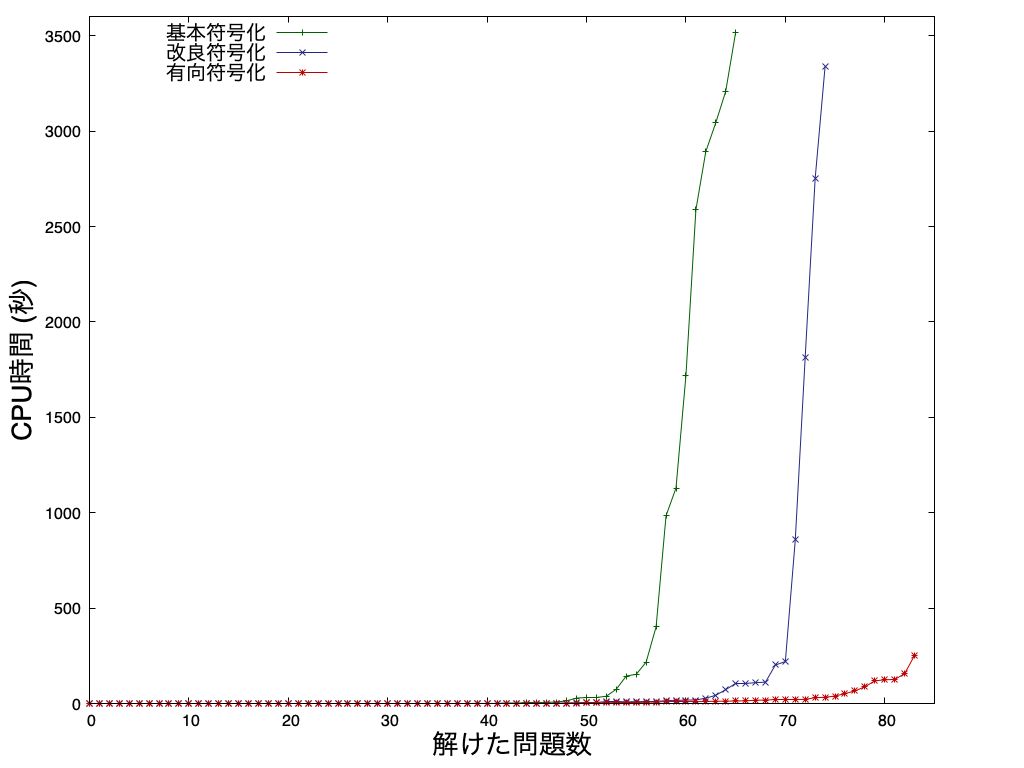
\includegraphics[scale=0.25]{fig/cactus_hq.png}
 \end{figure}

\begin{itemize}
 \item 有向符号化は,他の符号化と比較して,より多くの問題(84/85問)を高速に解いている.
\end{itemize}\vfill
\end{frame}
%%%%%%%%%%%%%%%%%%%%%%%%%%%%%%%%%%%%%%%%%%%%%%%%%%
%% 配電網遷移問題
%%%%%%%%%%%%%%%%%%%%%%%%%%%%%%%%%%%%%%%%%%%%%%%%%%
\begin{frame}{~}
 \LARGE \centering
 \structure{\bf 配電網遷移問題}
\end{frame}
%
\begin{frame}[noframenumbering]{配電網遷移問題の定式化}
  \begin{itemize}
  \item 配電網問題の変数集合
    $\boldsymbol{x} = \{x_1,x_2,\ldots,x_n\}$
    に対して,ステップ$t~\geq 0$での各変数の値を表す変数集合
    $\boldsymbol{x}^{t} = \{x_1^t,x_2^t,\ldots,x_n^t\}$を導入.
  \item スタート状態から$\ell$ステップ遷移した後の各変数の値
    $\boldsymbol{x}^{\ell}$が,ゴール状態を満足するかを判定するため,
    論理式$\varphi_{\ell}$を構成する.
  \end{itemize}
  \begin{block}{}\centering\vskip-1em
  \begin{align*}
  \varphi_{\ell} &= S(\boldsymbol{x}^0)  & S: \textrm{スタート状態を表す論理式} \\
  &\land \bigwedge_{t=0}^{\ell} C(\boldsymbol{x}^t) & C: \textrm{トポロジ制約,電流制約を表す論理式} \\
  &\land \bigwedge_{t=1}^{\ell} T(\boldsymbol{x}^{t-1},\boldsymbol{x}^{t}) 
   & T: \textrm{遷移制約を表す論理式} \\
  &\land G(\boldsymbol{x}^\ell)  & G: \textrm{ゴール状態を表す論理式}
  \end{align*}
  \end{block}
  \begin{itemize}
  \item {$\varphi_{\ell}$}が充足可能の場合,
    ステップ長$\ell$の到達可能な遷移系列が存在する
    ことを意味する.
  \end{itemize}
\end{frame}
%%%%%%%%%%%%%%%%%%%%%%%%%%%%%%%%%%%%%%%%%%%%%%%%%%
%% 提案アプローチ
%%%%%%%%%%%%%%%%%%%%%%%%%%%%%%%%%%%%%%%%%%%%%%%%%%
\begin{frame}{ASPを用いた配電網遷移問題の解法} 
  \begin{alertblock}{}\centering
    配電網遷移問題に対して,制限された長さの遷移系列
    \begin{align*}
    \varphi_{\ell} = S(\boldsymbol{x}^0)  
    \land \bigwedge_{t=0}^{\ell} C(\boldsymbol{x}^t) 
    \land \bigwedge_{t=1}^{\ell} T(\boldsymbol{x}^{t-1},\boldsymbol{x}^{t}) 
    \land G(\boldsymbol{x}^\ell)  
        \end{align*}
    を論理プログラムとして表現し,ASP システムを用いて\\
   実行することにより,到達可能性の検査を行う.
  \end{alertblock}\vfill
  \begin{itemize}
   \item $\varphi_{\ell}$が\structure{\bf 充足可能}の場合,
         ステップ長$\ell$の\structure{\bf 到達可能}な遷移系列が存在.
   \item $\varphi_{\ell}$が\structure{\bf 充足不能}の場合,
         ステップ長$\ell$では\structure{\bf 到達不能}.
   \item 到達不能の場合,$\ell$を増加させた論理プログラムを再構成し,
         繰り返し ASP システムを実行.
  \end{itemize}
\end{frame}
%%%%%%%%%%%%%%%%%%%%%%%%%%%%%%%%%%%%%%%%%%%%%%%%%%
%% 提案アプローチ
%%%%%%%%%%%%%%%%%%%%%%%%%%%%%%%%%%%%%%%%%%%%%%%%%%
\begin{frame}{配電網遷移問題のASP符号化}
% \begin{alertblock}{}
%  \centering
%  配電網遷移問題を解くASP符号化を2種類考案
% \end{alertblock}
% \vfill
   \begin{block}{シングルショット符号化}
    \begin{itemize}
     \item $\varphi_{\ell}$をそのまま1つの論理プログラムとして記述.
     \item 配電網問題のASP符号化の自然な拡張.
    \end{itemize}
   \end{block}
     \begin{itemize}
      \item ステップ長$\ell$を増加させながら,
            $\varphi_{\ell}$を繰り返し構成し解く.
      %\item 長所: 実装が単純である.
      \item 短所: 学習節が再利用できない.
      \item 短所: ASPシステムを毎回起動するオーバーヘッドが大きい.
     \end{itemize}
    \begin{alertblock}{マルチショット符号化}
     \begin{itemize}
      \item $\varphi_{\ell}$を,$S(\boldsymbol{x}^{0})$を表す\code{base}部,
            $C(\boldsymbol{x}^{t})$,$T(\boldsymbol{x}^{t-1},\boldsymbol{x}^{t})$
            を表す\code{step(t)}部,
            $G(\boldsymbol{x}^{t})$を表す\code{check(t)}部に分けて記述.
     \end{itemize}
    \end{alertblock}
     \begin{itemize}
      \item % $S(\boldsymbol{x}^{0})$, $C(\boldsymbol{x}^{t})$,
            % $T(\boldsymbol{x}^{t-1},\boldsymbol{x}^{t})$, $G(\boldsymbol{x}^{t})$
            % を動的に追加・削除しながら,
            $\varphi_{\ell}$をインクリメンタルに構成しながら解くことが可能.
      \item 長所: 学習節の再利用が可能.ASPシステムの起動は1回のみ.
      \item 短所: 現状では,デバックしにくい.
     \end{itemize} 
\end{frame}
%%%%%%%%%%%%%%%%%%%%%%%%%%%%%%%%%%%%%%%%%%%%%%%%%%
%% 実験内容--遷移問題
%%%%%%%%%%%%%%%%%%%%%%%%%%%%%%%%%%%%%%%%%%%%%%%%%%
\begin{frame}{実験概要}
  \renewcommand{\thefootnote}{\fnsymbol{footnote}}
  \setcounter{footnote}{1}
 提案するASP符号化の性能の評価実験を行った.
  \vfill
  \begin{itemize}
  \item \structure{\bf 比較するASP符号化:}
    \begin{itemize}
    \item シングルショット符号化
    \item マルチショット符号化
    \end{itemize}
  \item \structure{\bf ベンチマーク問題:} 全1000問
    \begin{itemize}
    \item DNET \footnote{https://github.com/takemaru/dnet}
      で公開されている実用規模の配電網問題 (\structure{\bf fukui-tepco},
      スイッチ数 468,変電所の数 72,許容電流 300A)をベース
    \item 実行可能解の中から,スタート状態を10個,ゴール状態を100個を
          ランダムに抽出し,それらを組み合わせて生成
    \end{itemize}
  \item \structure{\bf ASPシステム:} \textit{clingo-5.4.0} $+$ \textit{trendy}
   \item \structure{\bf 制限時間:} 10分/問
  \item \structure{\bf 実験環境:} Mac mini,3.2GHz Intel Core i7,64GBメモリ
  \end{itemize}
\end{frame}
%%%%%%%%%%%%%%%%%%%%%%%%%%%%%%%%%%%%%%%%%%%%%%%%%%
%% 実験結果--遷移問題
%%%%%%%%%%%%%%%%%%%%%%%%%%%%%%%%%%%%%%%%%%%%%%%%%%
\begin{frame}{実験結果:平均CPU時間の比較}
 \vfill
 \centering
 \vskip -2ex
 \scalebox{0.8}{\begin{tabular}{ccrrr}
 \rowcolor[RGB]{0,96,0}
\color{white}最短ステップ長 & \color{white}問題数 
     & \multicolumn{1}{c}{\color{white}シングルショット} 
         & \multicolumn{1}{c}{\color{white}マルチショット} 
             & \multicolumn{1}{c}{\color{white}シングル/マルチ} \\
 \rowcolor[RGB]{230,239,230}
1 & 6 & 1.677 & \alert{1.035} & 1.620 \\
 \rowcolor[RGB]{196,230,196}
2 & 62 & 3.507 & \alert{1.608} & 2.180 \\
 \rowcolor[RGB]{230,239,230}
3 & 189 & 6.089 & \alert{2.155} & 2.826 \\
 \rowcolor[RGB]{196,230,196}
4 & 312 & 9.294 & \alert{2.734} & 3.399 \\
 \rowcolor[RGB]{230,239,230}
5 & 280 & 13.338 & \alert{3.361} & 3.968 \\
 \rowcolor[RGB]{196,230,196}
6 & 130 & 18.303 & \alert{4.165} & 4.394 \\
 \rowcolor[RGB]{230,239,230}
7 & 21 & 24.483 & \alert{5.086} & 4.814 \\
\noalign{\hrule height 0.5pt}
 \rowcolor[RGB]{196,230,196}
計 & 1000 & 76.691 & \alert{20.114} & 3.807 \\
\end{tabular}

}
 \vfill
\begin{itemize}
 \item 1000問全ての到達可能性を判定でき,全て到達可能であった.
 \item 今回生成した問題のうち,最長で最短ステップ数は7であった.
 \item マルチショットは,シングルショットと比較して,全ての
	   問題をより高速に解いており,\alert{\bf 平均で3.8倍の高速化}を実現している.
\end{itemize}
\end{frame}
%%%%%%%%%%%%%%%%%%%%%%%%%%%%%%%%%%%%%%%%%%%%%%%%%%
%% まとめ
%%%%%%%%%%%%%%%%%%%%%%%%%%%%%%%%%%%%%%%%%%%%%%%%%%
\begin{frame}{まとめと今後の課題}
 \begin{alertblock}{}
  \centering
  配電網遷移問題に対して,ASPを用いた解法を提案した.
 \end{alertblock}
 \vfill
  \begin{enumerate}
   \item \structure{\bf 配電網問題のASP符号化の考案}
         \begin{itemize}
          \item トポロジ制約のASP符号化として,\textbf{基本符号化},\textbf{改良符号化},
                \\ \alert{\bf 有向符号化} の3種類を考案.
          \item 電気制約として,電流制約のASP符号化を考案.
         \end{itemize}
   \item \structure{\bf 配電網遷移問題のASP符号化の考案}
         \begin{itemize}
          \item \textbf{シングルショット符号化}と\alert{\bf マルチショット符号化}の2種類を考案.
          \item 配電網問題のASP符号化の自然な拡張である.
         \end{itemize}
   \item \structure{\bf 実用規模の問題を含むベンチマークによる評価実験}
         \begin{itemize}
          \item 実用規模の問題である\textsf{fukui-tepco}をもとに,
                配電網遷移問題ベンチマークを1000問作成.
          \item \textbf{マルチショット符号化}は,
                \alert{\bf 約3.8倍の高速化}を実現.
         \end{itemize}
  \end{enumerate}
 \vfill
 \begin{exampleblock}{今後の課題}
\begin{itemize}
 \item 電流制約だけでなく電圧制約も含む配電網遷移問題への拡張
 \item 完全な問題は非線形な制約を含むため,ASP Modulo Theoriesを用いた解法を検討
\end{itemize}
 \end{exampleblock}
\end{frame}

%###########################################################
%##### 補助スライド ########################################
%###########################################################

%%%% 補助スライド

\begin{frame}{~}
 \centering
 - 補足用 -
\end{frame} 

\begin{frame}{補足 : スマートグリッド}
 \begin{itemize}
  \item \structure{スマートグリッド}とは,電力の供給側,需要側において双方向の
		やり取りを可能にする次世代の\structure{賢い}電力網である.
  \item 従来と違い,通信技術の発達により,使用状況などを
		リアルタイムに把握することが可能となった.
  \item その時に応じた最適な配電網を構成し,制御するといったことが考えられている.
		\begin{itemize}
		 \item 電力需要の変化による,配電ロスの少ない構成.
		 \item 自然エネルギーによる発電量の変動を補う構成.
		\end{itemize}
  \item ASP言語の表現力や拡張性が,こうした条件の追加に活用できる可能性がある.
 \end{itemize}
\end{frame}

%%%%%%%%%%%%%%%%%%%%%%%%%%%%%%%%%%%%%%%%%%%%%%%%%%
%% 電気制約
%%%%%%%%%%%%%%%%%%%%%%%%%%%%%%%%%%%%%%%%%%%%%%%%%%
\begin{frame}{補足 : 電気制約}
 \begin{itemize}
  \item \alert{電気制約}は,送電する電流$\cdot$電圧の適正範囲を保証する制約.
  \begin{itemize}
   \item 供給経路の各区間で許容電流を超えない.
   \item 電気抵抗による電圧降下が許容範囲を超えない.
   \item etc.
  \end{itemize}
  \item 電流と電圧が影響し合う\structure{実数ドメイン上の制約}によって表される.
		% \begin{itemize}
		%  		 \item 送電システム上の条件など.
		% \end{itemize}
  \item 実数ドメイン上の制約は,純粋なASPのみで扱うのは\alert{困難}.
		\begin{itemize}
		 \item 緩和問題として,変電所から供給できる家庭の数に上限をつける.
		 \item ASPMT技術により,ASPで得られた解について,
			   背景理論ソルバーと連携して実数ドメイン上の制約を調べる.
		\end{itemize}
 \end{itemize}
\end{frame}


%%%%%%%%%%%%%%%%%%%%%%%%%%%%%%%%%%%%%%%%%%%%%%%%%%
%% 基礎化
%%%%%%%%%%%%%%%%%%%%%%%%%%%%%%%%%%%%%%%%%%%%%%%%%%
\begin{frame}{補足 : ASPシステム}
 
 \vspace{-0.5cm}

 \begin{figure}[htbp]
  \centering
  %%%%%%%%%%%%%%%%%%%%%%%%%%%%%%%%%%%%%%%%%%%%%%%%%%
%% 基礎化の流れの図
%%%%%%%%%%%%%%%%%%%%%%%%%%%%%%%%%%%%%%%%%%%%%%%%%%
\begin{tikzpicture}

 \definecolor{edge}{RGB}{38,38,134}
 \definecolor{node}{RGB}{220,220,249}

 \definecolor{alert_edge}{RGB}{191,0,0}
 \definecolor{alert_node}{RGB}{249,200,200}

 \definecolor{ex_edge}{RGB}{0,96,0}
 \definecolor{ex_node}{RGB}{230,239,230}

 \def\nodespace{2.4cm}

 \tikzset{block/.style={rectangle, thick, draw=edge, fill=node, text width=3cm, 
 text centered, rounded corners, text width=2cm, minimum height=1.5cm}};

 \tikzset{alertblock/.style={rectangle, thick, draw=alert_edge, fill=alert_node, 
 text width=3cm, text centered, rounded corners, text width=1.5cm, minimum height=1.2cm}};

 \node[block](ikkai){一階ASP\\プログラム};

 \node[rectangle,rounded corners, thick, draw=ex_edge, fill=ex_node, 
 right=0.22*\nodespace of ikkai, minimum width=6cm, minimum height=3cm, 
 text centered, label=ASPシステム](sys){};

 \node[block, right=\nodespace of ikkai](meidai){命題ASP\\プログラム};
 \node[block, right=\nodespace of meidai](ASP){解集合};

 \node[right=0.6*\nodespace of ikkai, text width=1.5cm, 
 text centered, text=red, anchor=south](){基礎化\\ソルバー};
 \node[right=0.4*\nodespace of meidai, text width=1.5cm, 
 text centered, text=red, anchor=south](){解集合\\ソルバー};

 
 \foreach \u / \v / \n in {ikkai/meidai,meidai/ASP}
 \draw [thick,->] (\u) to (\v);

\end{tikzpicture}
 \end{figure}

 \vspace{-0.5cm}

 \begin{exampleblock}{}
  \begin{enumerate}
   \item 一階ASPプログラムを基礎化ソルバーによって,
		 命題ASPプログラムに\alert{基礎化}する.
   \item 命題ASPプログラムについて,SAT技術を応用した解集合ソルバーが解集合を探索する.
  \end{enumerate}
 \end{exampleblock}

\end{frame}


%%%%%%%%%%%%%%%%%%%%%%%%%%%%%%%%%%%%%%%%%%%%%%%%%%
%% ASPのコード
%%%%%%%%%%%%%%%%%%%%%%%%%%%%%%%%%%%%%%%%%%%%%%%%%%
\begin{frame}[fragile]{補足 : 基本符号化のASPプログラム}
 \begin{exampleblock}{}
  \begin{center}
   %%%%%%%%%%%%%%%%%%%%%%%%%%%%%%%%%
   \lstinputlisting[numbers=left,%
   basicstyle=\ttfamily\tiny]{code/srf1.lp}
   %%%%%%%%%%%%%%%%%%%%%%%%%%%%%%%%% 
  \end{center}
 \end{exampleblock}
\end{frame}

\begin{frame}[fragile]{補足 : 改良符号化のASPプログラム}

 \begin{exampleblock}{}
  \begin{center}
   %%%%%%%%%%%%%%%%%%%%%%%%%%%%%%%%%
   \lstinputlisting[numbers=left,%
   basicstyle=\ttfamily\tiny]{code/srf2.lp}
   %%%%%%%%%%%%%%%%%%%%%%%%%%%%%%%%% 
  \end{center}
 \end{exampleblock}

\end{frame}



\end{document}
%%% Local Variables:
%%% mode: japanese-latex
%%% TeX-master: t
%%% End:

